\section{Stellwerkstechnik}\label{text:Grundlagen:Stellwerkstechnik}

Mit der Eröffnung der ersten Eisenbahnstrecke 1825 in England begann ein neues Zeitalter. Die Eisenbahn ermöglichte es, Personen und Güter schneller und effizienter zu transportieren als je zuvor. Mit zunehmendem Verkehr auf der Schiene stieg auch die Notwendigkeit der Sicherung der Fahrwege. Dieser Abschnitt behandelt die Grundlagen der Stellwerkstechnik, wie sie bei realen Eisenbahnen eingesetzt wird. Dabei wird zunächst der theoretische Hintergrund erläutert. Anschließend werden die drei geläufigsten technischen Umsetzungen vorgestellt. Diese sind mechanische, Relais- und elektronische Stellwerke. Zuletzt wird auf die neueste Entwicklung, das digitale Stellwerk, eingegangen.

\subsection{Sicherung des Schienenverkehrs}\label{text:Grundlagen:Stellwerkstechnik:Sicherung-des-Schienenverkehrs}

In den Anfangsjahren der Eisenbahn wurde die Notwendigkeit von Sicherungssystemen schnell deutlich. Ein großer Fortschritt war der Einsatz von Telegraphen, um Zugbewegungen zwischen Bahnhöfen zu koordinieren --- ein Verfahren, das heute noch unter dem Namen \textit{Zugleitbetrieb} angewandt wird. Jedoch war dieses Verfahren nicht ausreichend, um die Sicherheit der Fahrwege zu gewährleisten. So kam es immer wieder zu schweren Unfällen mit vielen Toten. Dies führte in der Folge zur Entwicklung elaborierter Sicherungssysteme, die letztlich in die heutige Stellwerkstechnik mündeten.

\subsubsection*{Streckenblock}\label{text:Grundlagen:Stellwerkstechnik:Sicherung-des-Schienenverkehrs:Streckenblock}

Das mit Abstand wichtigste Konzept der Sicherungstechnik ist der Streckenblock. Hierbei handelt es sich zunächst um ein theoretisches Konstrukt, das später mit technischen Mitteln angewandt wird. Eine Zugstrecke wird in logische Abschnitte unterteilt, die \textit{Streckenblöcke} oder \textit{Blockabschnitte}. Hierbei gilt die wichtigste Regel der Sicherungstechnik: in einem Streckenblock darf sich immer nur ein Zug zur selben Zeit befinden.

\subsubsection*{Signale}\label{text:Grundlagen:Stellwerkstechnik:Sicherung-des-Schienenverkehrs:Signale}

Ein Signal ist ein technisches Mittel, um den Zugverkehr zu steuern. Konkret sichert es die Einfahrt in einen Streckenblock ab. Signale können in zwei wesentlichen Bauarten ausgeführt sein: als Formsignal und als Lichtsignal. Formsignale sind die ältere Bauart und werden heute nur noch selten eingesetzt. Sie bestehen aus einem Mast, an dem ein oder mehrere bewegliche Arme angebracht sind. Die Stellung der Arme gibt die Bedeutung des Signals an. Lichtsignale sind die heute übliche Bauart. Sie bestehen aus einem Mast, an dem mehrere Lichter angebracht sind. Die Bedeutung des Signals wird durch die Anordnung und Farbe der Lichter angezeigt. In \autoref{abb:Grundlagen:Stellwerkstechnik:Signale} sind beispielhaft ein Form- und ein Lichtsignal dargestellt.

% https://de.wikipedia.org/wiki/Datei:Ks_Signal_NALB.jpg
% https://de.wikipedia.org/wiki/Datei:Formsignale.jpg
\begin{margin}
    \begin{figure}
    \centering

    \begin{subfigure}{0.45\textwidth}
        \centering
        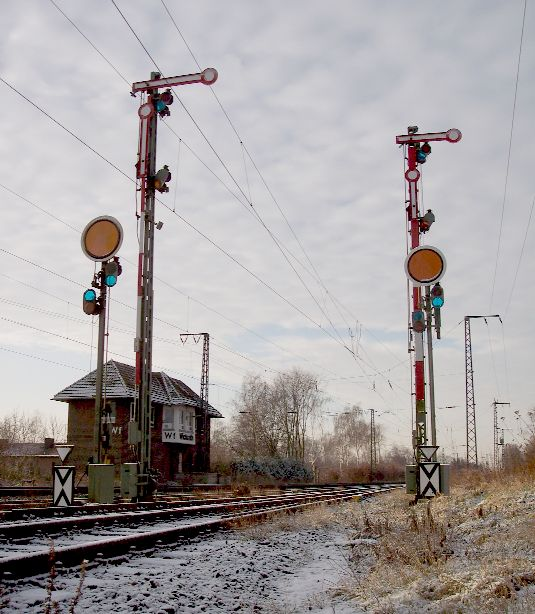
\includegraphics[width=\textwidth]{Assets/Images/2-Grundlagen/Formsignale.jpg}
        \caption{Formsignale}\label{abb:Grundlagen:Stellwerkstechnik:Formsignale}
    \end{subfigure}

    \begin{subfigure}{0.45\textwidth}
        \centering
        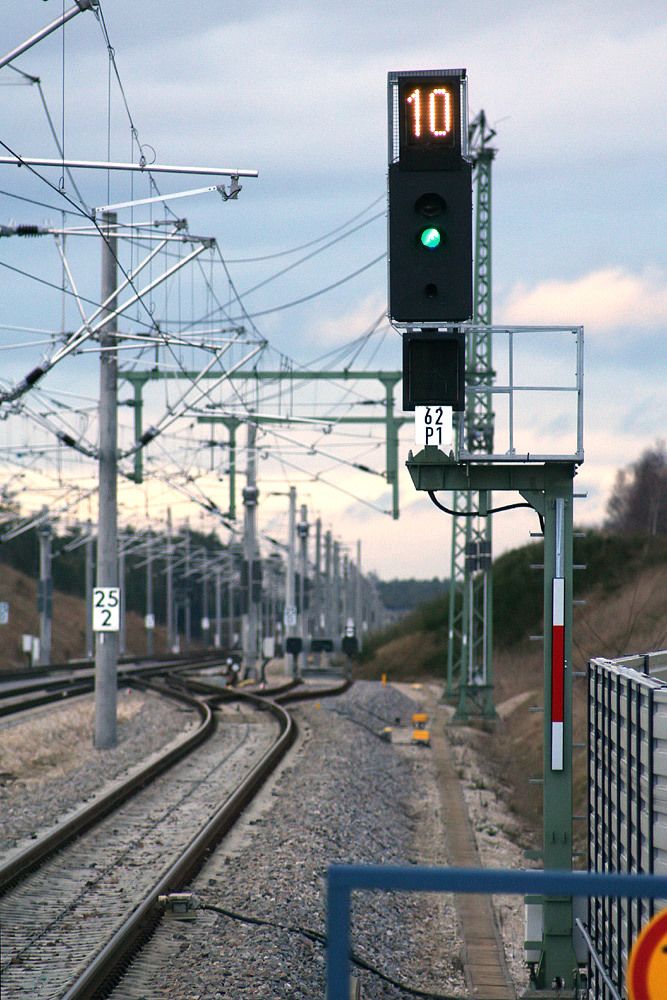
\includegraphics[width=\textwidth]{Assets/Images/2-Grundlagen/Ks-Signal.jpg}
        \caption{Lichtsignal}\label{abb:Grundlagen:Stellwerkstechnik:Lichtsignal}
    \end{subfigure}

    \caption{Beispiele für deutsche Eisenbahnsignale}\label{abb:Grundlagen:Stellwerkstechnik:Signale}
    \end{figure}
\end{margin}

In Deutschland sind mehrere Signalsysteme im Einsatz. Ein Signalsystem beschreibt die Bedeutung der Signale und die zugehörigen Signalbilder. Wie Ampeln im Straßenverkehr können Eisenbahnsignale einem Zug die Weiterfahrt erlauben oder verwehren. Außerdem können zulässige Höchstgeschwindigkeiten und die Richtung, in die ein Fahrweg eingestellt ist, angezeigt werden. Da diese Arbeit ihren Fokus nicht auf Signalisierung legt, soll auf dieses Thema nicht weiter eingegangen werden.

\subsubsection*{Weichen}\label{text:Grundlagen:Stellwerkstechnik:Sicherung-des-Schienenverkehrs:Weichen}

\subsubsection*{Fahrstraße}\label{text:Grundlagen:Stellwerkstechnik:Sicherung-des-Schienenverkehrs:Fahrstrasse}

\subsection{Mechanische Stellwerke}\label{text:Grundlagen:Stellwerkstechnik:Mechanische-Stellwerke}

\subsection{Relaisstellwerke}\label{text:Grundlagen:Stellwerkstechnik:Relaisstellwerke}

\subsection{Elektronische Stellwerke}\label{text:Grundlagen:Stellwerkstechnik:Elektronische-Stellwerke}

\subsection{Digitale Stellwerke}\label{text:Grundlagen:Stellwerkstechnik:Digitale-Stellwerke}
